Ben Trout

2014-11-21

Building  

\begin{tabular}{|p{4cm}|p{6cm}|}
\hline
 Intake&
With the help of Filip I returned to the original idea with the intake at the front and the launcher behind it. We moved the launcher to the middle of the robot, but still with the same gear ratio and height of the ground. We put the intake back on the robot exactly where we had it when we had it there before: right at the front as low as possible (between the bar).
\\
\hline
Ramp&
Me and Matt were put incharge to make a ramp for our robot. We made a circle with radius 6in in a cardboard box and cut it out. We then drew tangent lines to opposit sides of the circle and conected the tangent lines. We cut these lines out making a square with a curve radius 6in going from one corner to the next. This will allow the ramp to have a nice smooth curve that the ball can easily travel up. Me and Matt then put supports on the back and front of these two cureved pieces attatching them together. We finally got a piece of cardstock and taped it along the curved part of our cardboard sidese making a rigid and smooth ramp. 
\\
\hline
Claw&
One of the final pieces to our robot is the claw that will hook onto the rolling goal and drag it around with us as we launch balls into it. I had Matt head this, but helped a long the way. We got two servos that attach to the back of the robot that have a bar conected between them. Attatched to the bar is two claws perfectly spaced to hook into the holes on the rolling goals. The servos will bring the claws up allowing the robot to fit in the 18in by 18in box and then release them down when we are ready to hook into the rolling goal and drag it around with us. 
\\
\hline
\end{tabular}

\section*{Building Intake}
Once Alex finally returned he pointed out the flaws in having the intake and ball launcher being the same thing at the front of the robot. We need these two to be separate because the intake needs to be flexible to pick up balls of the wall while the launcher needs to be rigid to hit the balls up the ramp. We went back to our old plan which was very easy because we saved our original intake. Rebuilding the robot as we had it before was super easy. It was just a time game and Filip helped me put it back together as we had it before, only difference was our intake is the same as we had it when it was in the front of our robot. 

\section*{Ramp and Claw}
As the intake got done and Nick and Alex started to rewire me and Matt started to work on the ramp and claws. I had Matt do the ramp first time around while I finished the intake, but we only had regular paper at that time and the ramp was slanted as the curves weren't semetrical. As I finished up with the intake I helped Matt and we learned from our old mistakes. We made sure the circle was perfectly round and made sure our tangent lines were perfectly tangent, because if they weren't we'd have an angled ramp to one side like we had last time. We carefully cut out every piece and taped it all together. We then got cardstock instead of paper and used that for the ramp as it is sturdier and will last the impact of a ball going up it. As we finished the ramp we moved onto the claw. It is still in the very begining stages and we have no pictures right now as we're just messing around with the idea, and only have conceptual images in our heads of what it would look like. How I described it above is how it will most likely end up being. Right now it's a lot of messing around with different positions of the servos to make sure they pivot the claws up and down. 

\begin{center}
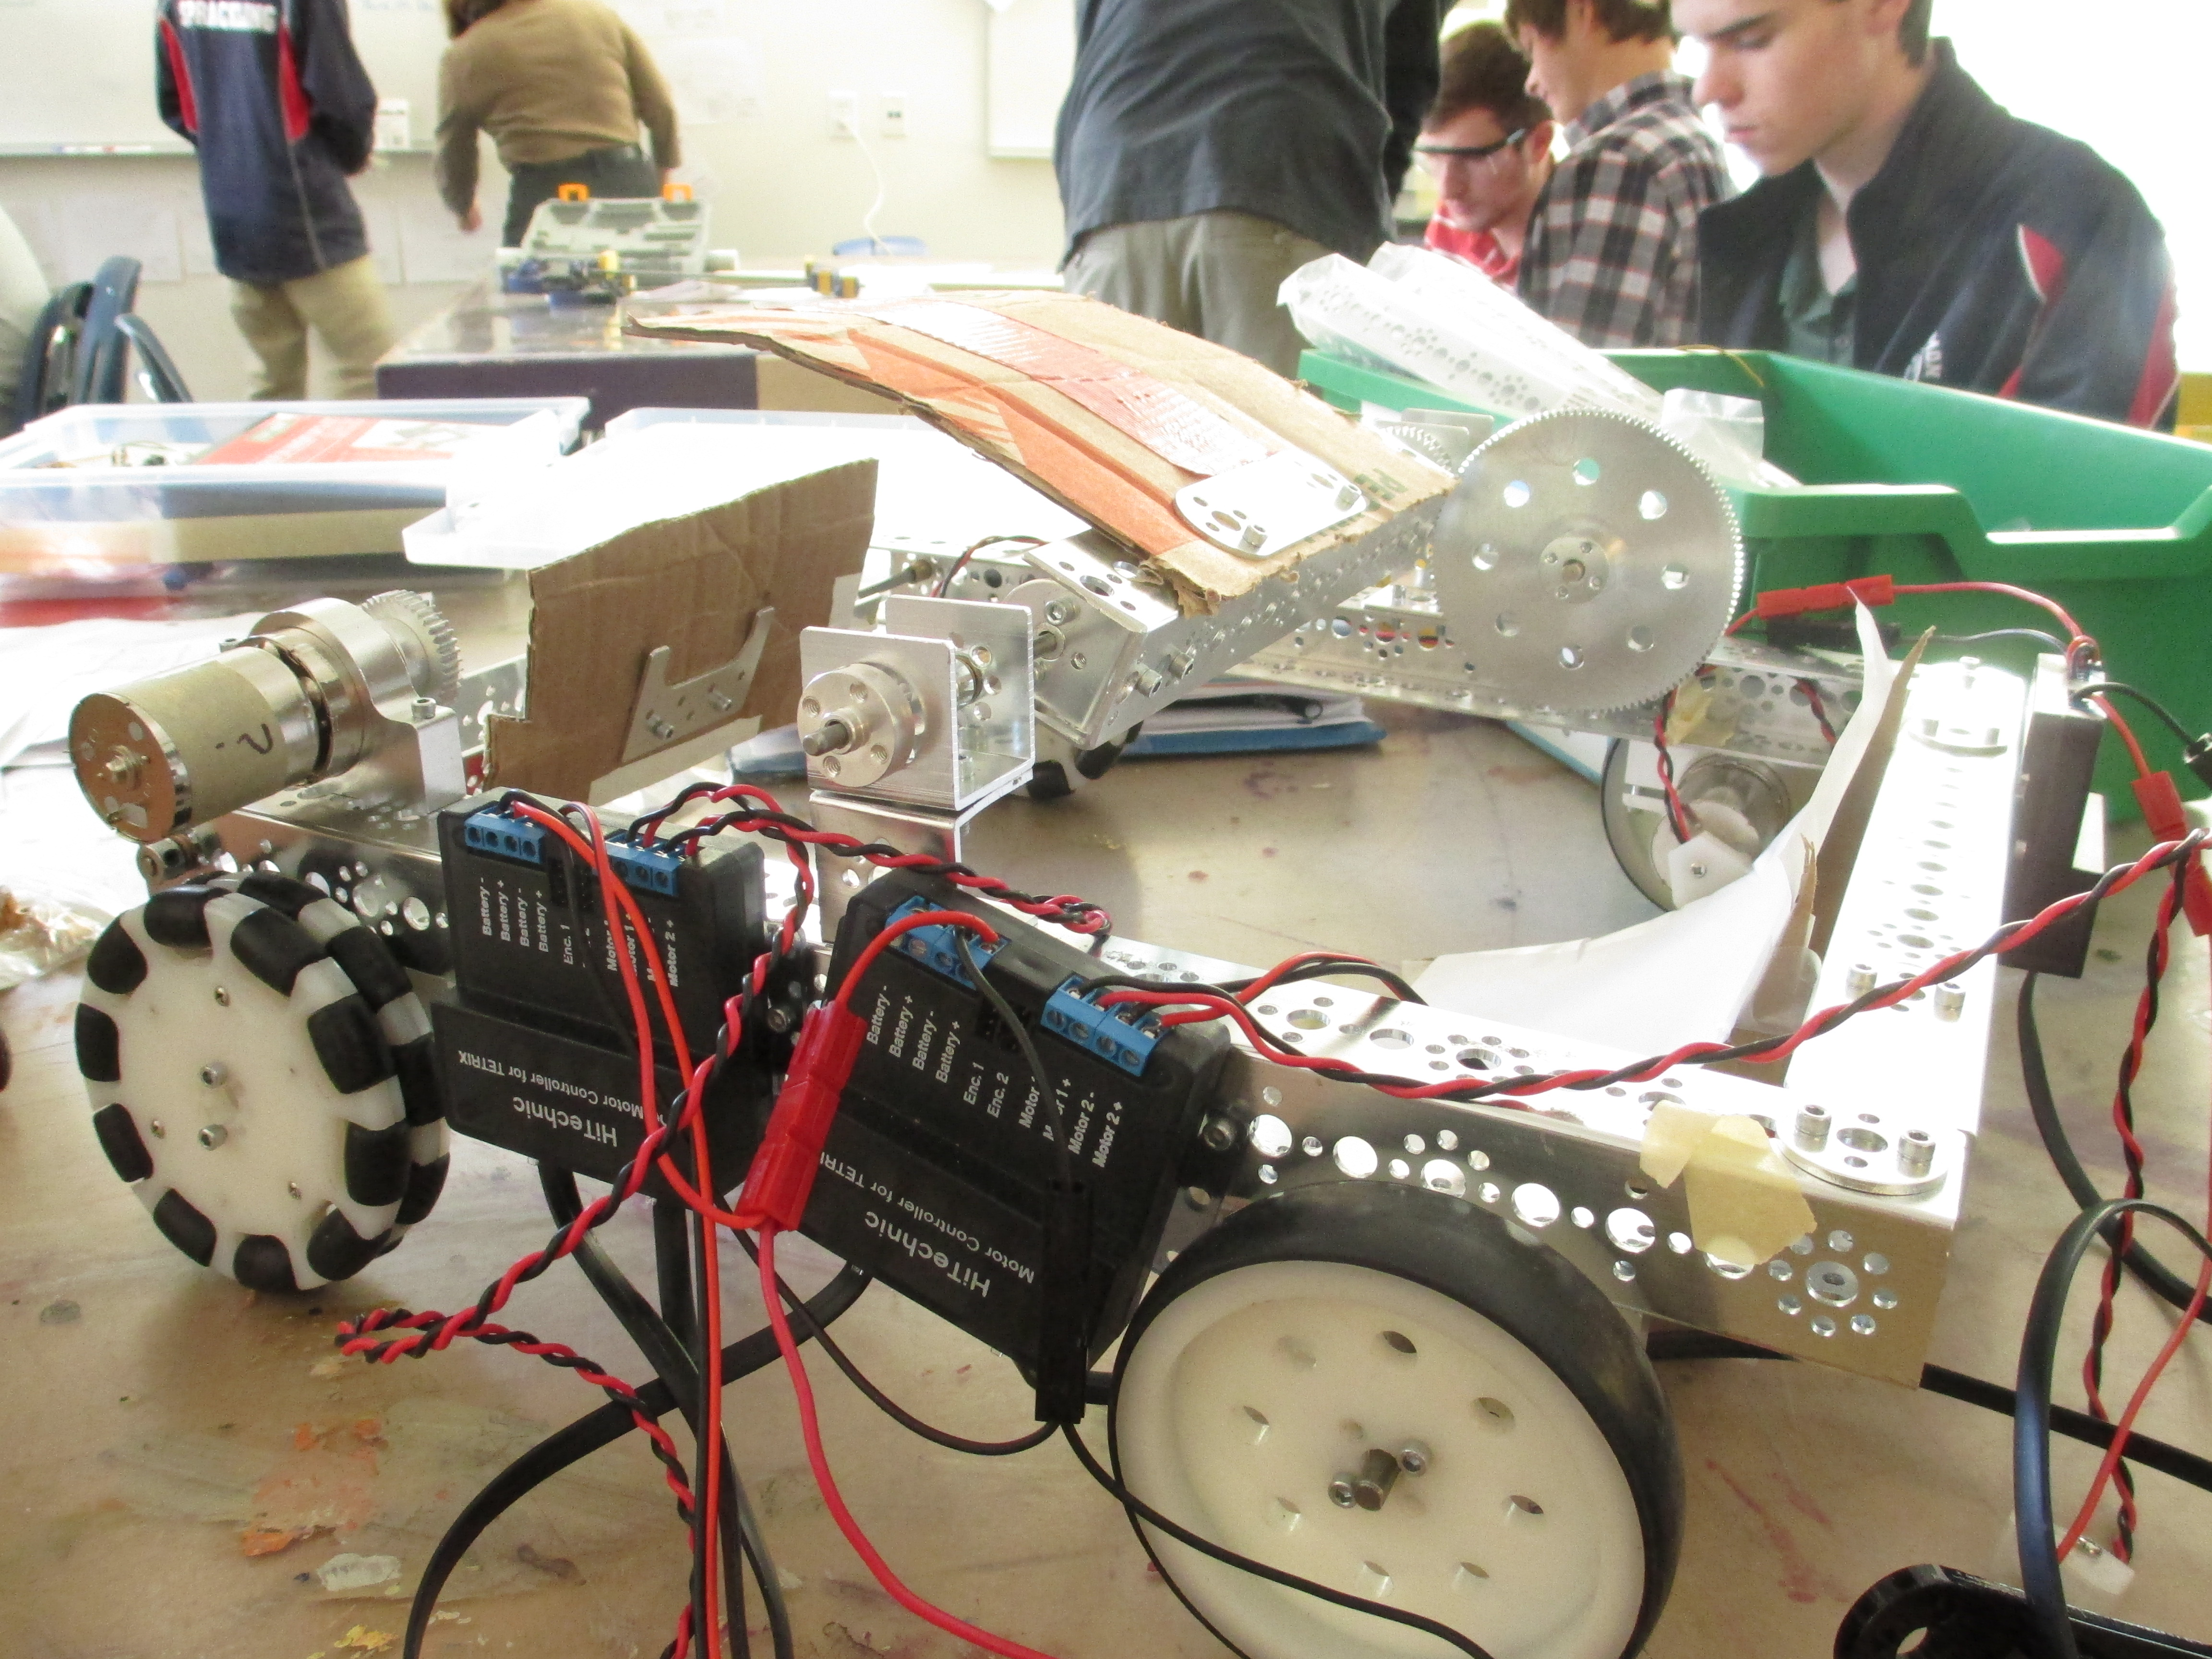
\includegraphics[width=10cm]{./Entries/Images/RobotDesignForNovemberTwentyFirstTwoThousandAndFourteenWithIntakeLauncherAndRampWiringIncludedILoveAlexHeIsTheBestNic.jpg}
\end{center}
